\section{Methodology}
\label{sec:methodology}

We describe the benchmark data provenance, translation pipeline, cross-lingual verifier architecture, label mapping scheme, and the risk calibration procedure for selective verification.

\begin{figure*}[t]
\centering
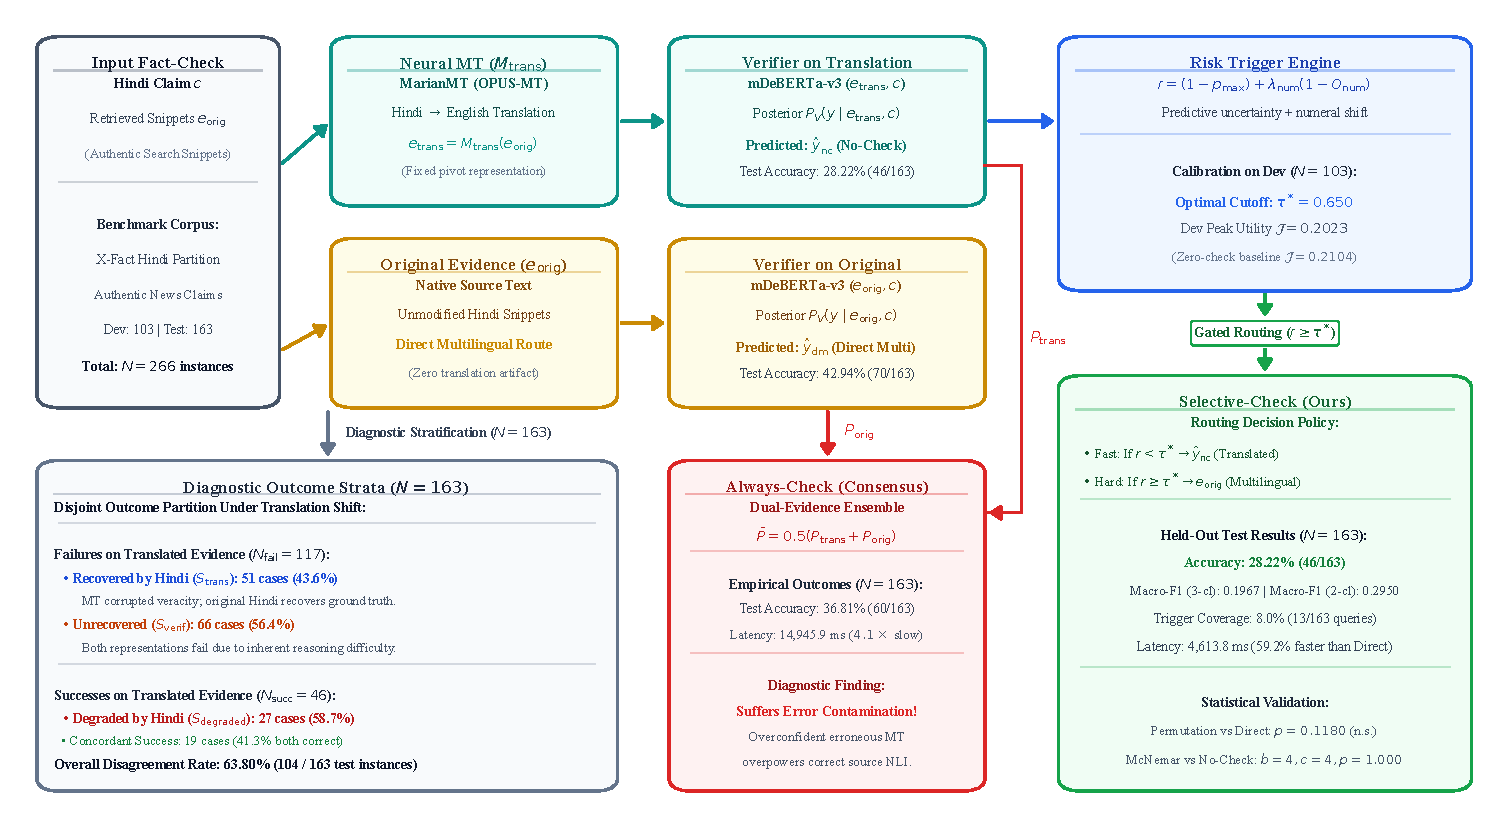
\includegraphics[width=0.92\textwidth]{figures/final/fig1_study_workflow.pdf}
\caption{System architecture and paired evaluation pipeline. Given an authentic Hindi claim and pre-retrieved Hindi evidence from X-Fact, the verifier (\texttt{mDeBERTa-v3-base}) is evaluated under four conditions: No-Check (translated English evidence), Direct Multilingual (original Hindi evidence), Always-Check (dual posterior consensus), and Selective-Check (risk-calibrated fallback).}
\label{fig:fig1_workflow}
\end{figure*}

\subsection{Benchmark Data and Pre-Retrieved Evidence}
We conduct our empirical evaluation on the Hindi partition of the X-Fact benchmark \citep{gupta-srikumar-2021-xfact}. X-Fact consists of authentic real-world claims crawled from international fact-checking platforms (such as \emph{Vishvas News}, \emph{Jagran Fact Check}, and \emph{Factly}), accompanied by scraped evidence snippets and multi-class veracity verdicts assigned by professional fact-checkers.

\paragraph{Evidence Snippet Grounding.}
Critically, X-Fact provides pre-retrieved evidence snippets collected by human fact-checkers to substantiate their verdict. We explicitly note that \emph{our experimental setup does not evaluate upstream search engine retrieval or dense passage retrieval}. By holding the pre-retrieved evidence text constant, we eliminate retrieval noise as an uncontrolled confounder and strictly isolate the effect of evidence language representation on downstream verifier inference.

\paragraph{Split Provenance.}
The official X-Fact Hindi partition comprises $N=266$ total verified instances, partitioned into a development set ($N=103$) and a held-out evaluation set ($N=163$). As detailed in Section~\ref{sec:exp_setup}, we utilize the development partition exclusively for hyperparameter tuning and risk threshold calibration, reserving the $N=163$ split for diagnostic evaluation.

\subsection{Machine Translation Pipeline}
To generate translated evidence passages ($e_{\text{trans}}$), we employ \texttt{Helsinki-NLP/opus-mt-hi-en} \citep{tiedemann-thottingal-2020-opus}, a standard MarianMT encoder-decoder architecture widely deployed for open-source Hindi-to-English machine translation. The model operates with standard sentence-piece tokenization, a beam search width of 4, and a maximum sequence length of 512 tokens. Claims are preserved in their original phrasing or paired directly with translated evidence according to standard cross-lingual verification practice.

\subsection{Multilingual Verifier Architecture}
For claim veracity scoring, we deploy \texttt{MoritzLaurer/mDeBERTa-v3-base-xnli-multilingual-nli-2mil7} \citep{laurer-etal-2024-less}. This model builds upon the 12-layer \texttt{mDeBERTa-v3-base} backbone \citep{he-etal-2021-deberta}, utilizing disentangled attention and enhanced masked language modeling pre-trained on 100 languages. It is fine-tuned on a composite corpus of 2.7 million natural language inference examples spanning MNLI, ANLI, FeverNLI, and multilingual XNLI \citep{conneau-etal-2020-unsupervised}.

\paragraph{Premise-Hypothesis Structuring.}
Following standard automated fact-checking conventions \citep{thorne-etal-2018-fever,shcharbakova-etal-2025-scale}, we frame evidence verification as an NLI classification task:
\begin{align}
    \text{Premise} &= e \in \{e_{\text{orig}}, e_{\text{trans}}\}, \\
    \text{Hypothesis} &= c.
\end{align}
The model produces unnormalized logits $g_\theta(c, e) = [z_{\text{contra}}, z_{\text{neutral}}, z_{\text{entail}}]^\top$, which are mapped via softmax to posterior probabilities.

\paragraph{Label Mapping Scheme.}
We map the 3-class NLI output space to the X-Fact verification taxonomy:
\begin{equation}
    y = \begin{cases}
        \textsc{Contradicted} & \text{if } \arg\max = \text{contradiction}, \\
        \textsc{Insufficient\_Evidence} & \text{if } \arg\max = \text{neutral}, \\
        \textsc{Supported} & \text{if } \arg\max = \text{entailment}.
    \end{cases}
\end{equation}

\subsection{Selective Cascade and Risk Calibration}
\label{sec:risk_calibration}
The Selective-Check condition is designed to minimize inference compute and latency by evaluating only the translated evidence ($e_{\text{trans}}$) when confidence is high, falling back to original Hindi evidence ($e_{\text{orig}}$) via hard routing only when a test-time risk score indicates potential translation or reasoning failure.

\paragraph{Risk Scoring Formulation.}
We formulate the risk metric $r(c, e_{\text{trans}}, e_{\text{orig}}) \in [0, 1]$ as an additive combination of verifier predictive uncertainty and surface-level numeral distortion:
\begin{equation}
    r = \big(1 - \max_{y \in \mathcal{Y}} P_\theta(y \mid c, e_{\text{trans}})\big) + \lambda_{\text{num}} \cdot \big(1 - \operatorname{Overlap}_{\text{num}}(c, e_{\text{trans}})\big),
    \label{eq:risk_score}
\end{equation}
where $\max_y P_\theta(y \mid c, e_{\text{trans}})$ is the maximum softmax probability (MSP) on translated evidence, and $\operatorname{Overlap}_{\text{num}}(c, e_{\text{trans}}) \in [0, 1]$ measures the Jaccard overlap of Arabic and Devanagari numerals appearing in the claim and translated passage. The hyperparameter $\lambda_{\text{num}} \ge 0$ scales the numeral penalty. When $r \ge \tau^*$, the system executes hard routing to original Hindi evidence ($\hat{y}_{\text{dm}}$), while falling back to dual posterior consensus ($\hat{y}_{\text{ac}}$) is evaluated as an explicit ablation.

\paragraph{Development Threshold Tuning.}
To avoid data contamination, the decision threshold $\tau^*$ and weight $\lambda_{\text{num}}$ were selected via a grid search exclusively over the $N=103$ development partition. Optimization targeted a cost-sensitive utility objective:
\begin{equation}
    J(\tau) = \operatorname{Macro-F1}_3(\tau) - 0.15 \cdot \operatorname{Coverage}(\tau),
\end{equation}
where $\operatorname{Coverage}(\tau) \in [0, 1]$ denotes the fraction of queries routed to original-language verification.

\begin{figure}[t]
\centering
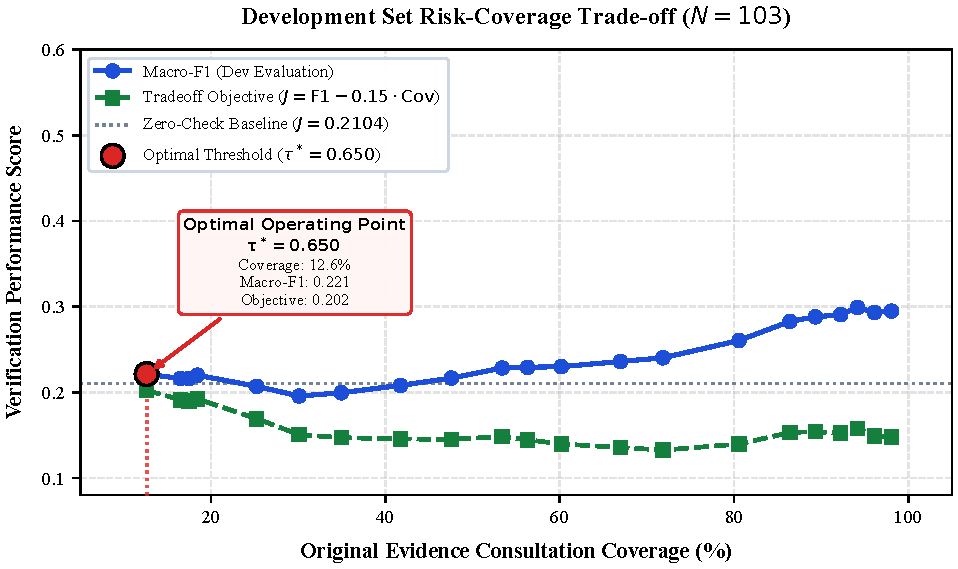
\includegraphics[width=\columnwidth]{figures/final/fig2_risk_coverage_tradeoff.pdf}
\caption{Risk-coverage trade-off and utility optimization on the $N=103$ development split. The optimal operating threshold is identified at $\tau^* = 0.650$ ($J = 0.2023$). The zero-check baseline utility achieves $J = 0.2104$.}
\label{fig:fig2_tradeoff}
\end{figure}

Grid search over $\tau \in [0.10, 0.90]$ in increments of $0.05$ identified an optimal operating point at $\tau^* = 0.650$ and $\lambda_{\text{num}} = 0.20$ (Figure~\ref{fig:fig2_tradeoff}). Crucially, on development data, the zero-check baseline achieved utility $J = 0.2104$, whereas the peak cascade utility reached only $J = 0.2023$. This development diagnostic demonstrated prior to test evaluation that the selective cascade faced a steep trade-off between coverage cost and classification gain.
